\secput{poly}{Polytopal Range Queries}

% introduce how to use meta-algorithm to handle irregular range queries,
% including, right triangular queries, arbitrary triangular queries, to
% arbitrary polygonal queries

In this section, we use one simple example of non-orthogonal query to
illustrate the real power of meta-algorithm. The examples in this section
is for right triangle that rectilinear to the axes and hypotenuse of slope
$\angle 45^{\circ}$ degree.  How to extend the methodology to arbitrary
triangular query in $2$-D grid and how to extend it to higher-dimensional
grids are our future work.

\subsecput{triangle}{Triangular Query in $2$-D grid}

\begin{figure*}[!ht]
\centering
\subfigure[Initial algorithm for right triangular query in $2$-D grid]{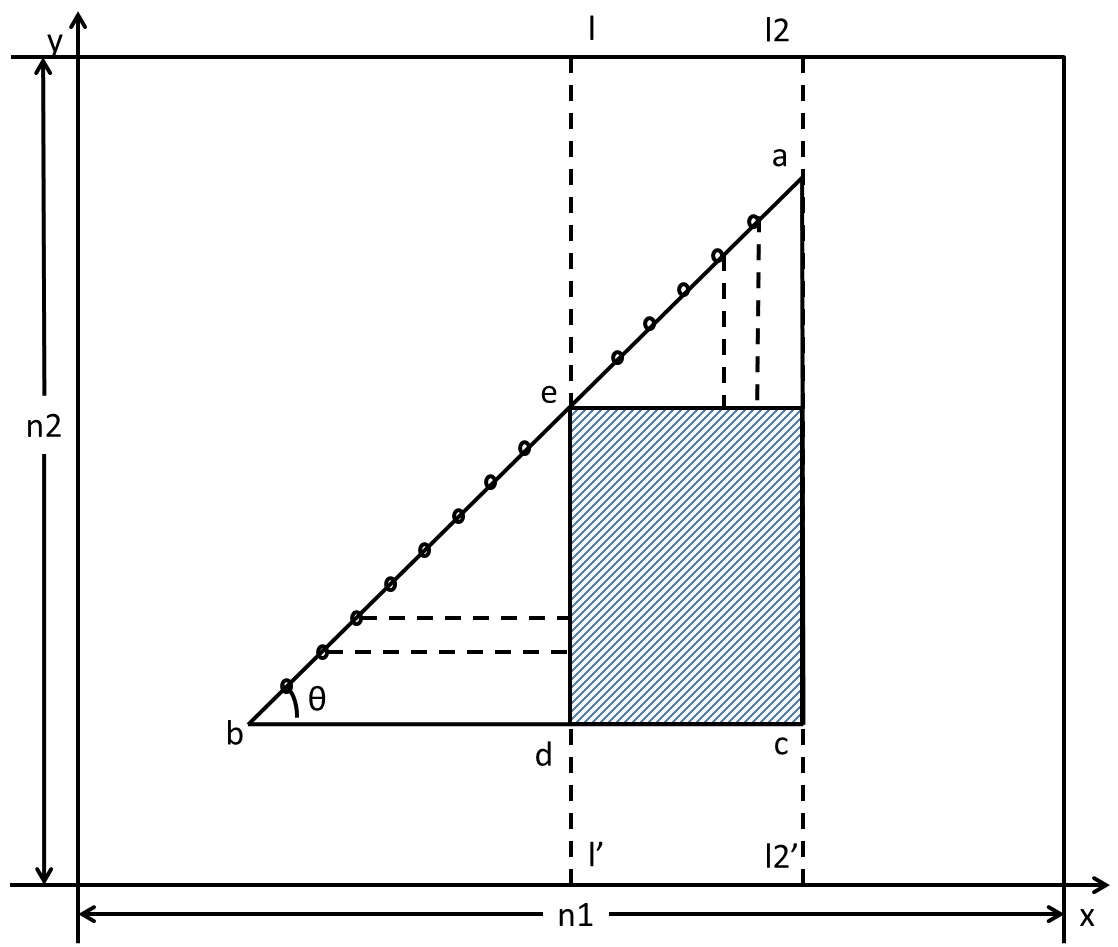
\includegraphics[clip,width=3in]{figures/init_right_triangle.eps}
\label{fig:init-right-triangle}}
\hfill
%\hspace{0.01cm}
\subfigure[Meta-algorithm for right triangular query in $2$-D grid]{\includegraphics[clip,width=3in]{figures/meta_right_triangle.eps}
\label{fig:meta-right-triangle}
}
\caption{Initial and meta-algorithm for right triangular query in $2$-D grid}
\label{fig:right-triangle}
\end{figure*}

\subsubsecput{rightTri}{Right Triangular Query in $2$-D grid}

\subsubsubsecput{initRightTri}{Initial algorithm for right triangular query in $2$-D grid}
As shown in \figref{init-right-triangle}, the initial algorithm
for processing right triangles in $2$-D grid is very similar to that
processing rectangles.  Suppose the slope $\angle\theta$ is given as in
\figref{init-right-triangle}, we have following initial algorithm:

\begin{enumerate}
\item Without loss of generality, let's suppose we do the partition on 
  dimension $\id{x}$. The first cut partition the entire grid into evenly
  two parts by a center line $\overline{\id{ll'}}$.
\item For any point on the left side of the center line, do the same data
  reduction as in orthogonal range preprocessing. Let's name it 
  \defn{rectangular reduction}
\item For any point on the right side of the center line, it will perform
  two passes of data reduction and stores two reduced values respectively.
  One is the normal \defn{rectangular reduction}, the other is something
  we name \defn{triangular reduction}. For example: for point $\id{a}$
  in \figref{init-right-triangle}, since it's on the right-hand side of
  the center line, it needs to do both \defn{rectangular reduction} and
  \defn{triangular reduction}. The details of \defn{triangular reduction}
  are as follows: 
    \begin{itemize}
    \item Conceptually draw a line of slope $\angle\theta$, which will 
      cross the center line $\overline{\id{ll'}}$ at point $\id{e}$.
    \item From $\id{e}$, draw a horizontal line $\overline{\id{ef}}$
      parallel to axis $\id{x}$.
    \item Reduce the value of point $\id{a}$ from horizontal line 
      $\overline{\id{ef}}$. 
    \end{itemize} 
\item Store the reduced values from \defn{rectangular reduction} on the
  left side and \defn{triangular reduction} on the right side along
  slanted line of angle ($\angle\theta$) in a $1$-D grid, e.g. store reduced
  values along line $\overline{\id{ab}}$ in a $1$-D grid.
\item Recursion on the left and right grids completes the preprocessing
  for any right triangular query in the grid with slope $\angle\theta$.
\end{enumerate}

% to improve: the time bound of this naive \defn{triangular reduction}
\begin{theorem}
The preprocessing space is $\Theta(n_1 n_2 \log n_1 \log n_2)$, the
corresponding time bound is $\Theta(n_2 n_1^2 \log n_1)$, provided that 
$\tan \theta$ is a preprocessing time constant.
\end{theorem}

\begin{IEEEproof}
Apparently, for \defn{rectangular reduction} it has exactly the same space
and time bound as in orthogonal range preprocessing. The difference lies in
\defn{triangular reduction}.

Take \figref{init-right-triangle} as an example, for point $\id{a}$,
the time complexity of \defn{triangular reduction} equals the length
of line $\overline{\id{af}}$.  If we suppose the coordinates of point
$\id{a}$ is $(x, y)$, then length of $\overline{\id{af}}$ equal to
$(x - n_1/2) \cdot \tan \theta$.  Combining all the length along line
$\overline{\id{ae}}$ we have $\Sigma_{x=n_1/2}^{n_1} (x - n_1/2) \cdot
\tan \theta = n_1^2/8 \cdot \tan \theta = \Theta(n_1^2 \tan \theta$. Due
to the slope $\angle \theta$, there are $n_2 - n_1/2 \cdot \tan \theta$
number of such slanted lines at this recursion level.  Summing them up,
we have $(n_2 - n_1/2 \cdot \tan \theta) \cdot n_1^2/8 \cdot \tan \theta =
\Theta(n_2 n_1^2 \tan \theta) = \Theta(n_2 n_1^2)$, provided that $\tan
\theta$ is a preprocessing time constant. Since there are $\log n_1$
recursion levels, summing up the time bound in all recursion levels
yields time bound $\Theta(n_2 n_1^2 \log n_1)$
\end{IEEEproof}

\begin{corollary}
The query overhead of initial algorithm for right triangular query in
$2$-D grid is $\mathcal{Q}_{2, right\_triangle, 0} = 3-\oplus$
\end{corollary}

\begin{IEEEproof}
Similar to the orthogonal range query, first we need to locate the
recursion level the right triangle range crosses, the cost of which
is omitted in our simple arithmetic model. After spotting the recursion
level, any right triangles that span across the center line of the recursion
level can be answered by two $1$-D queries. One along slanted $1$-D grid, 
another on the right side of center line. 

Still take \figref{init-right-triangle} as an example, suppose we are 
querying the partial sum in right triangle $\triangle \id{abc}$.
We will decompose the right triangular query into two $1$-D sub-queries, 
one of range $\overline{\id{ab}}$ along proper slanted $1$-D grid, 
another of range $\overline{\id{fc}}$ along line $\overline{\id{l_2l_2'}}$.
\end{IEEEproof}

\subsubsubsecput{metaRightTri}{Meta algorithm for Right Triangular Query in $2$-D grid}
The meta-algorithm for right triangular query is very similar to that
for rectangular query. The only difference comes at :
\begin{enumerate}
\item The $\id{input\_2D\_algo}$ is a $2$-D algorithm for right triangular 
  query.
\item The $\id{input\_1D\_algo}$ will be applied along both vertical line
  along one axis, and along slanted line with given slope $\angle \theta$.
\end{enumerate}

The detailed analysis is omitted in this extended abstract due to space 
limitation.

\subsubsecput{arbitraryTri}{Arbitrary Triangular Query in $2$-D grid}

\begin{figure*}[!ht]
\centering
\subfigure[Initial algorithm for arbitrary triangular query in $2$-D grid]{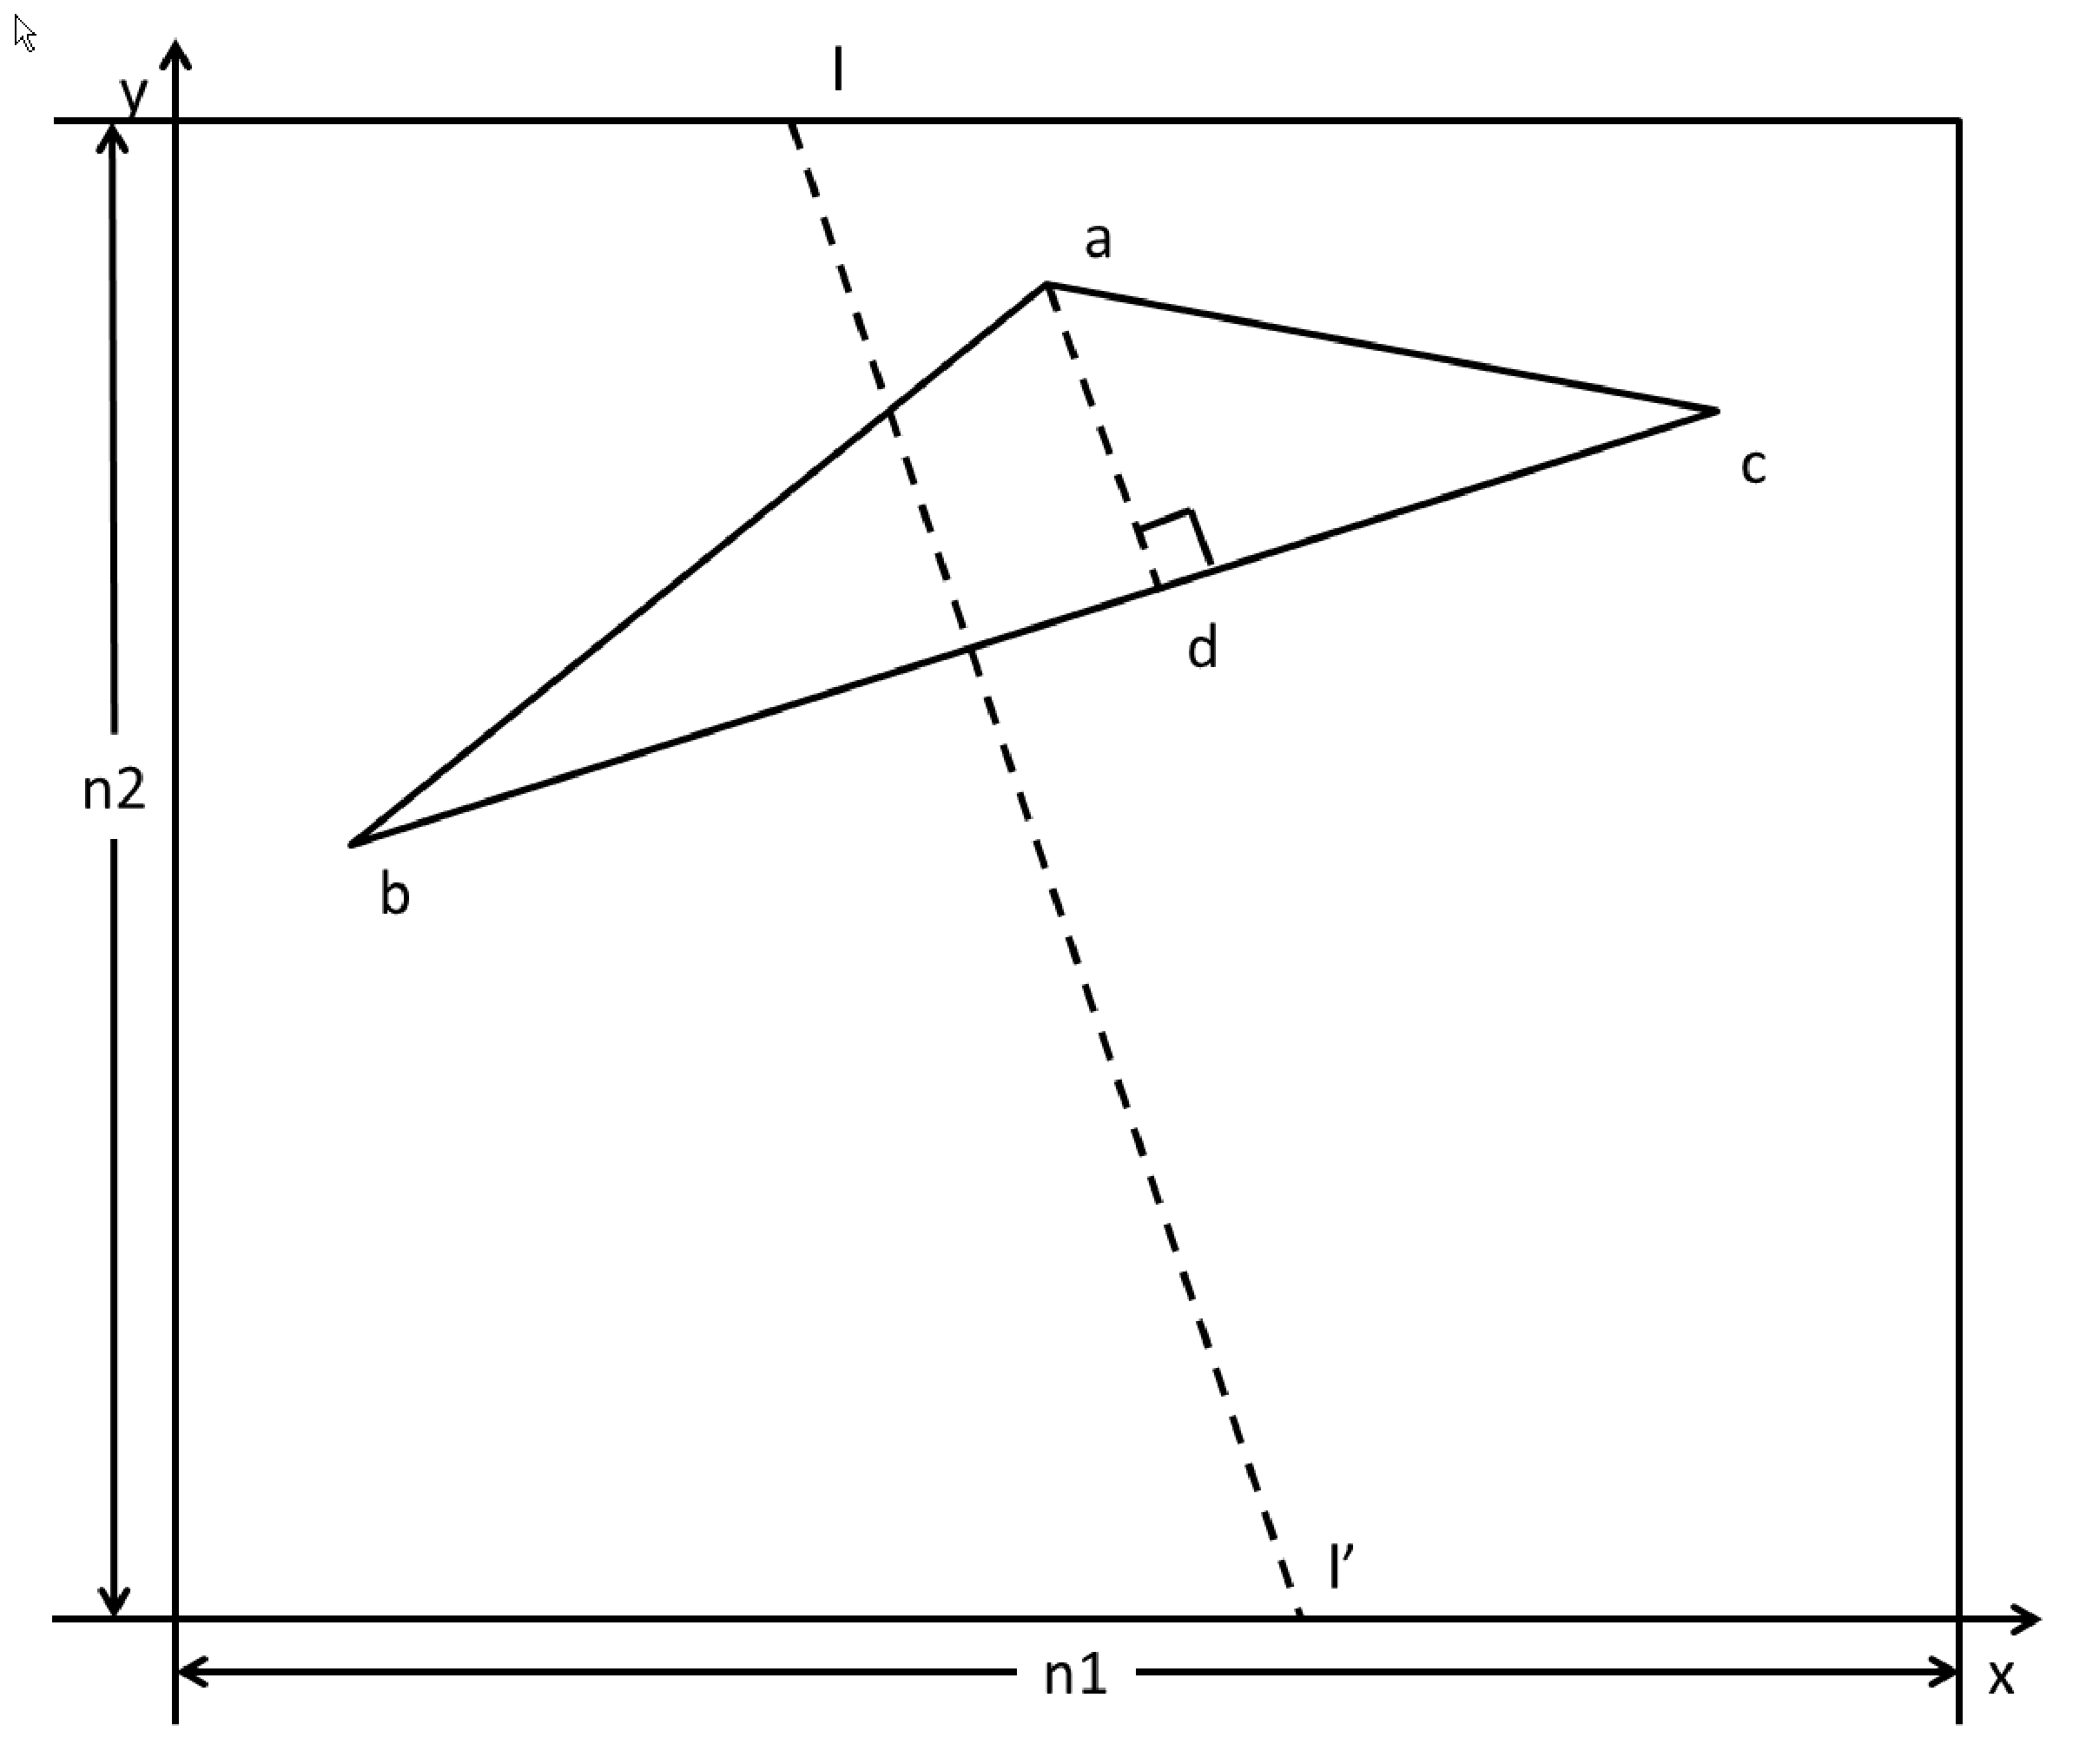
\includegraphics[clip,width=3in]{figures/init_arbitrary_triangle.eps}
\label{fig:init-arbitrary-triangle}}
\hfill
%\hspace{0.01cm}
\subfigure[Initial algorithm for arbitrary polygonal query in $2$-D grid]{\includegraphics[clip,width=3in]{figures/Polytopal_decomposition.eps}
\label{fig:meta-2D}
}
\caption{Initial algorithm for arbitrary triangular and polygonal query in $2$-D grid}
\label{fig:arbitraryTrianglePolygon}
\end{figure*}

The initial algorithm for arbitrary triangular query is illustrated in 
\figref{init-arbitrary-triangle}. The basic idea is:

\begin{enumerate}
\item For any triangles, it must have one angle larger than or equal to
  $60^{\circ}$ degree, draw from that point to the opposite line
  a perpendicular line, which must resides inside the triangle and
  partition the triangle into two right triangles. For example, in
  \figref{init-arbitrary-triangle}, point $\id{a}$ has an angle larger
  than $60^{\circ}$, draw a perpendicular line $\overline{\id{ad}}$
  its opposite line $\overline{\id{bc}}$.
\item Use the slope of the perpendicular line as the slope of center
  line that partition the entire $2$-D grid and partition the entire
  grid as the algorithm for right triangles. For example, in
  \figref{init-arbitrary-triangle}, we will use line $\overline{\id{ll'}}$
  as the center line to partition the entire grid.
\item Now any triangular query of the same three normals can be answered by
  combining the results of two right triangular sub-queries. For example,
  in \figref{init-arbitrary-triangle}, the triangular query of $\triangle
  \id{abc}$ can be answered by combining the results from two sub-queries
  on right triangles $\triangle \id{abd}$ and $\triangle \id{adc}$.
\item We claim that the above initial algorithm doesn't change any 
  asymptotic bound of the algorithm for right triangular query.
\end{enumerate}

\subsecput{polygon}{Polygon query in $2$-D grid}
The key issue in querying an arbitrary polygon range in a $2$-D grid lies
in how to decompose the polygon with given set of normals into a series
(constant number) of basic blocks. By basic blocks, we mean, rectangles
and triangles without changing or additional normals.

